\documentclass[12pt,a4paper]{report}
\usepackage[german]{babel}
\usepackage{graphicx}
\usepackage{listings}
\usepackage{amsfonts}
\usepackage{amsmath}
\graphicspath{ {images/} }
\hyphenation{Euklidischer}
\usepackage[square,numbers]{natbib}
\bibliographystyle{abbrvnat}

\usepackage{color}

\definecolor{mygreen}{rgb}{0,0.6,0}
\definecolor{mygray}{rgb}{0.5,0.5,0.5}
\definecolor{mymauve}{rgb}{0.58,0,0.82}

\lstset{ %
  backgroundcolor=\color{white},   % choose the background color;
  basicstyle=\footnotesize,        % the size of the fonts that are used for the code
  breakatwhitespace=false,         % sets if automatic breaks should only happen at whitespace
  breaklines=true,                 % sets automatic line breaking
  captionpos=b,                    % sets the caption-position to bottom
  commentstyle=\color{mygreen},    % comment style
  deletekeywords={...},            % if you want to delete keywords from the given language
  escapeinside={\%*}{*)},          % if you want to add LaTeX within your code
  extendedchars=true,              % lets you use non-ASCII characters; for 8-bits encodings only, does not work with UTF-8
  frame=single,	                   % adds a frame around the code
  keepspaces=true,                 % keeps spaces in text, useful for keeping indentation of code (possibly needs columns=flexible)
  keywordstyle=\color{blue},       % keyword style
  language=Octave,                 % the language of the code
  otherkeywords={*,...},           % if you want to add more keywords to the set
  numbers=left,                    % where to put the line-numbers; possible values are (none, left, right)
  numbersep=5pt,                   % how far the line-numbers are from the code
  numberstyle=\tiny\color{mygray}, % the style that is used for the line-numbers
  rulecolor=\color{black},         % if not set, the frame-color may be changed on line-breaks within not-black text (e.g. comments (green here))
  showspaces=false,                % show spaces everywhere adding particular underscores; it overrides 'showstringspaces'
  showstringspaces=false,          % underline spaces within strings only
  showtabs=false,                  % show tabs within strings adding particular underscores
  stepnumber=1,                    % the step between two line-numbers. If it's 1, each line will be numbered
  stringstyle=\color{mymauve},     % string literal style
  tabsize=2,	                   % sets default tabsize to 2 spaces
  title=\lstname                   % show the filename of files included with \lstinputlisting; also try caption instead of title
}

\begin{document}

\chapter*{Gliederung}
\begin{enumerate}
\item Einleitung
\item Grundlagen
    \begin{enumerate}
    \item Mustererkennung
        \begin{enumerate}
        \item Merkmalsbeschreibung
        \item Klassifikatoren
        \end{enumerate}
    \item Signalgewinnung / Gewinnung der Sensordaten
    \end{enumerate}
\item Anwendung / Beschreibung der Aufgabe und des Datensatzes
\item Konkrete Umsetzung
    \begin{enumerate}
    \item Datenvorverarbeitung
    \item Merkmalsberechnung auf Datens\"atze
    \item Anwendung der Klassifikatoren
    \item Absch\"atzung / Vergleich der Ergebnisse
    \end{enumerate}
\item Zusammenfassung
\end{enumerate}

\chapter{Mustererkennung}

\paragraph{}
Unter dem Begriff Mustererkennung versteht man die auomatische Verarbeitung und
Auswertung von Mustern und deren Zuordnung zu vorbestimmten Klassen. Die Muster%
erkennung setzt eine problemangepa\ss{}te Me\ss{}weterfassung voraus. Bild
\ref{fig:mustererkennung} zeigt die Struktur eines akustischen
Mustererkennungssytems.

\begin{figure}[ht]
\centering
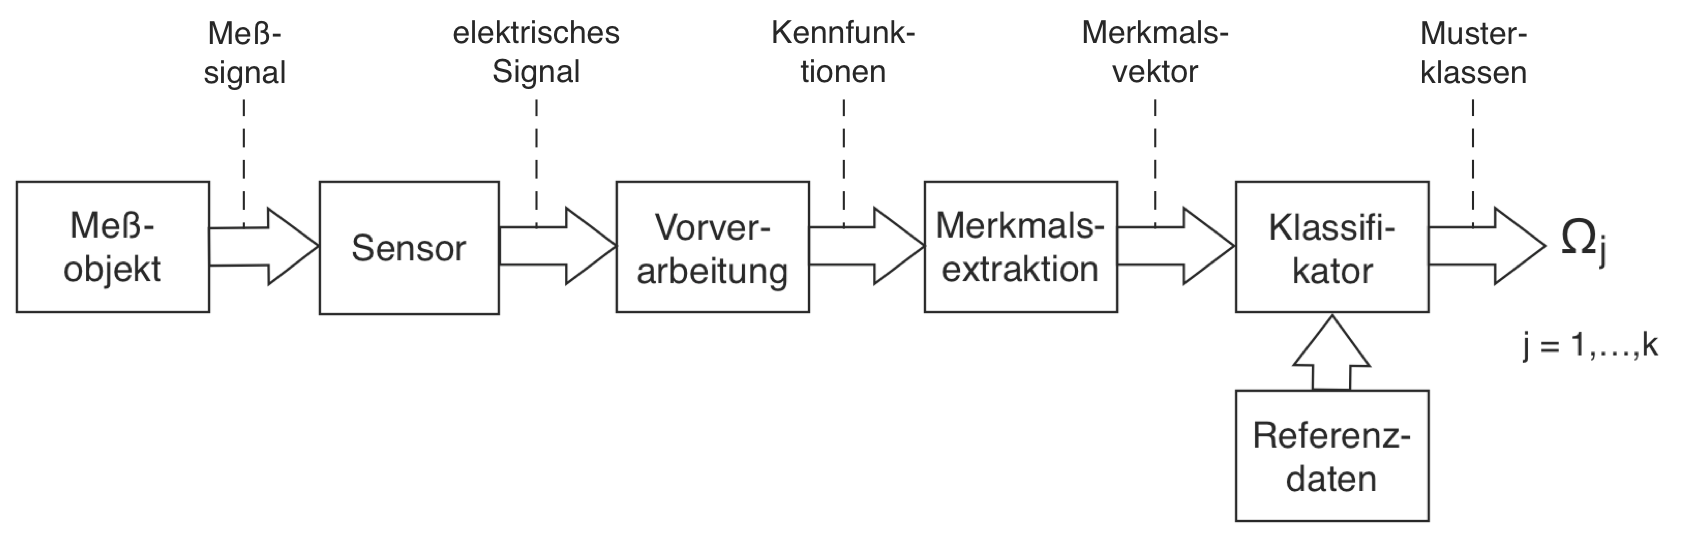
\includegraphics[width=1\textwidth]{mustererkennung}
\caption{Struktur der Mustererkennung}
\label{fig:mustererkennung}
\end{figure}

\paragraph{}
Das \textbf{Me\ss{}objekt} ist der zu erkennende Gegenstand. In der 
Ger\"auschdiagnose werden Me\"objekte nach einem bestimmten akustischen
Verhalten untersucht.

\paragraph{}
Der \textbf{Sensor} (Me\ss{}wertaufnehmer) wandelt die vom Me\ss{}objekt
ausgestrahlten mechanischen oder akustischen Schwingungen (Me\ss{}signale) in
elektrische Signale um. Wegen ihrer Unempfindlichkeit gegen\"uber
Umgebungsger\"auschen werden bevorzugt K\"orperschallaufnehmer f\"ur die
Me\ss{}werterfassung eingesetzt.

\paragraph{}
Durch die \textbf{Vorverarbeitung} wird ein Signal in eine f\"ur die weitere
Verarbeitung geeignetere Form gebracht. Sie beinhaltet im wesentlichen die
AD-Wandlung des analogen elektrischen Signals und die Transformation in
geeignete Kennfunktionen. Dabei mu\ss{} eine optimale Aussteuerung des
AD-Wandlers gew\"ahrleistet sein. Dementsprechend m\"ussen Verst\"arkungs-
bzw. D\"ampfungsma\ss{}nahmen durchgef\"uhrt werden. Au\ss{}erdem sind die
Bedingungen des Abtasttheorems zu erf\"ullen, was gegebenenfalls den Einsatz
eines Antialiasing-Filters erfoldert.

\paragraph{}
Auf der Stufe der \textbf{Merkmalsextraktion} werden aus den Kennfunktionen
zun\"achst Kennwerte ermittelt, die Beitr\"age zur Klassentrennung liefern
k\"onnen. Um den Merkmalen Chancengleichheit bez\"uglich der Klassentrennung
einzur\"aumen, erfolgt h\"aufig eine Kennwertnormierung (z.B. in den Werte%
bereich [0..1]). Eine weitere Hauptaufgabe der Merkmalsextraktion ist die
Auswahl der signifikantesten Merkmale hinsichtlich ihrer Klassentrennungs%
f\"ahigkeit, die eine Merkmalsselektion bedeutet. Mit der Auswahl der Merkmale
ist eine Datenreduktion (Merkmalsreduktion) verbunden. Zus\"atzlich kann eine
Merkmalsreduktion liefert schlie\ss{}lich Merkmalsvektoren, die als Komponenten
die verschiedenen Merkmale bzw. deren Transformation enthalten.

\paragraph{}
Der Merkmalsvektor wird dem \textbf{Klassifikator} zur Verf\"ugung gestellt.
Dieser allein ist f\"ur eine Klassifikation nicht ausreichend. Ein Muster%
erkennungssystem kann eine Erkennungsaufgabe nur dann automatisch l\"osen,
wenn es bestimmte Informationen \"uber das zu erkennende Objekt und die zu
differenzierenden Klassen besitzt. Der Klassifikator ben\"otigt also f\"ur die
Zuordnung des Me\ss{}objektes zu einer Lernphase zu berechnen sind. Die Art der
klassenspezifischen Information h\"angt vom verwendeten Klassifikatortyp ab. Je
nach Art der Entscheidungsfunktion kann es sich dabei um eine Stichprobe
vorklassifizierter Muster oder um Klassenrepr\"asentanten (Parameter) handeln,
die aus der Lernstichprobe berechnet werden. Falls keine Klassifikation eines
Me\ss{}objektes mit bestimmter Wahrscheinlichkeit m\"oglich ist, kann eine
R\"uckweisung erfolgen.\\
Um ein Urteil \"uber die Lernstichprobe zu bilden und die Eignung eines
Klassifikators f\"ur diese zu testen, wird die Lernstichprobe klassifiziert.
Dir Klassifikation der Lernmuster selbst, also der Proze\ss{} der Re%
klassifikation, liefert eine scheinbare Fehlerrate. Im Idealfall sollte
diese 0\% betragen. Diese sogenannte Reklassifikationsfehlerrate wird als
Akzeptanzma\ss{} daf\"ur angesehen, ob eine Lernstichprobe f\"ur die
Klassifikation unabh\"angiger Objekte geeignet ist.\\
Die Reklassifikationsfehlerrate ist nicht allein ausreichend, um die Leistung
der Mustererkennung mit dem gew\"ahlten Klassifikator zu beurteilen. Praktisch
geht man so vor, eine unabh\"angige Teststichprobe mit bekannter Klassen%
zugeh\"origkeit der Objekte neu zu klassifizieren. Dieser Vorgang wird \textbf{%
Testklassifikation} genannt. Die Fehlerrate der Testklassifikation ist ein
reales Fehlerma\ss{} f\"ur den eingesetzten Klassifikator und liegt in der Regel
h\"oher als die scheinbare Fehlerrate bei Reklassifikation. Damit l\"a\ss{}t
sich die Wirksamkeit eines Erkennungssystem beurteilen.

\begin{figure}[ht]
\centering
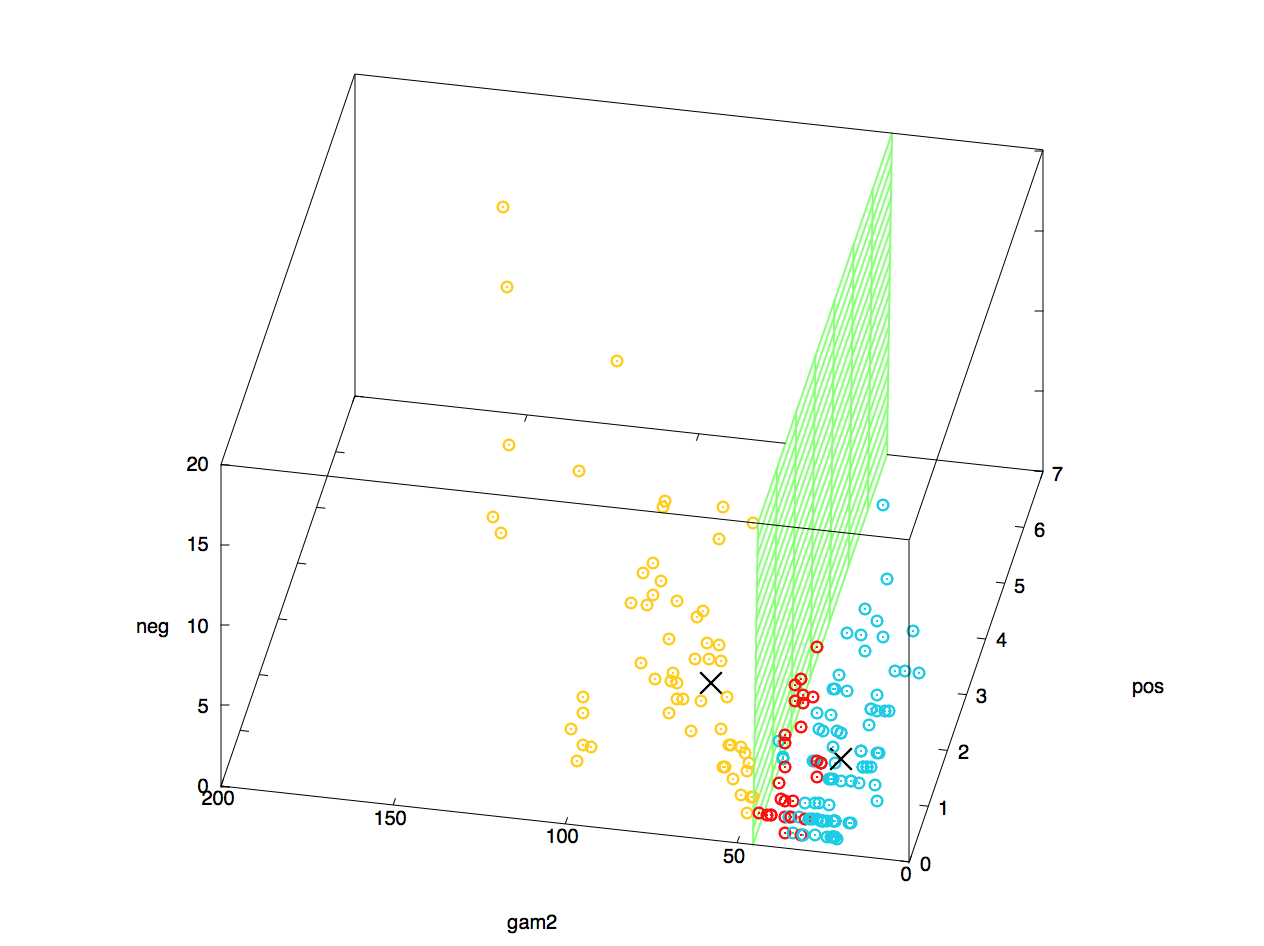
\includegraphics[width=1\textwidth]{mindestabstandEuklid}
\caption{Ergebnis der Pr\"ufung des Mindestabstand Klassifikators (Euklidischer
Abstand)}
\end{figure}

\begin{figure}[ht]
\centering
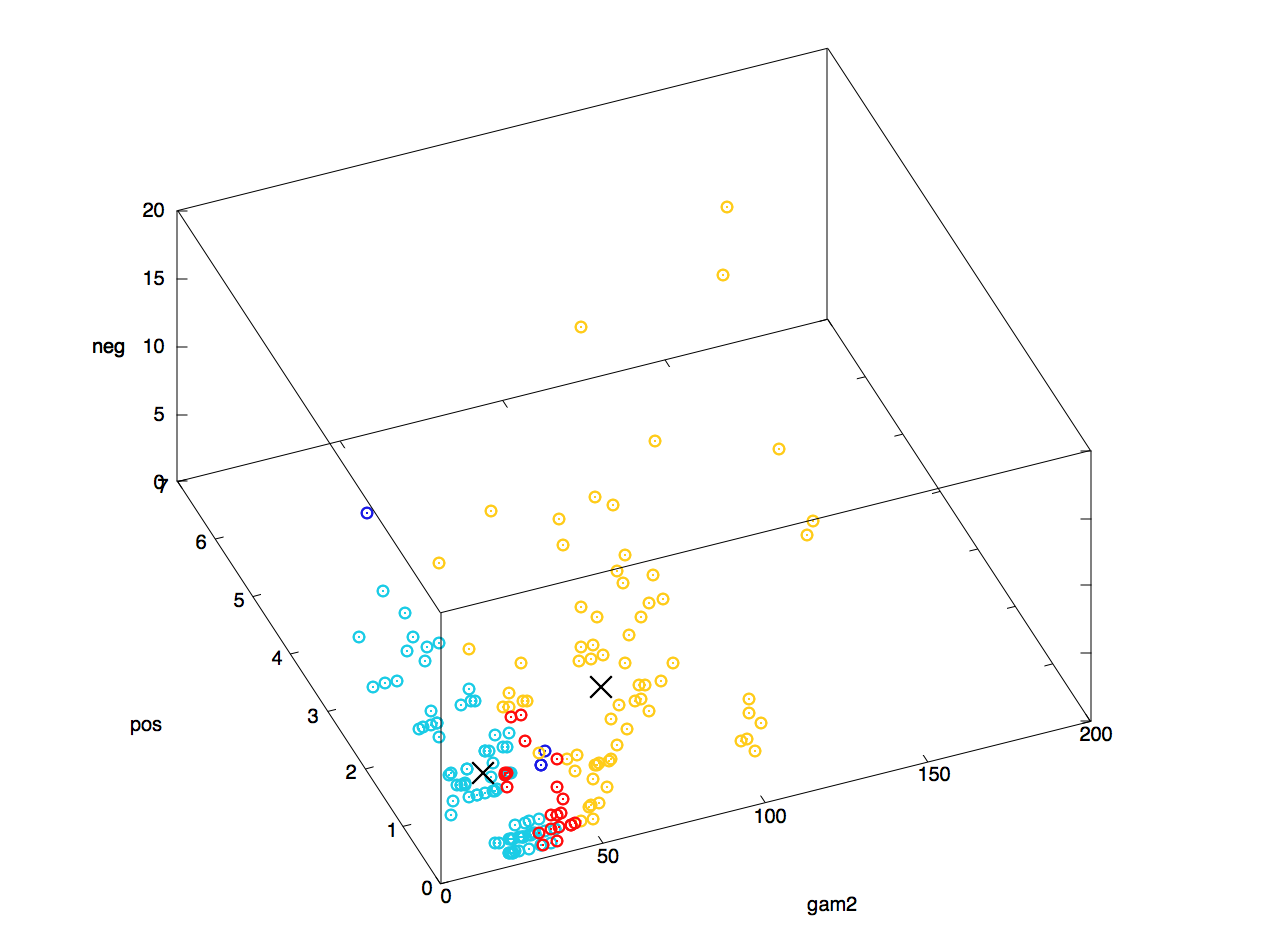
\includegraphics[width=1\textwidth]{mindestabstandMahalanobis}
\caption{Ergebnis der Pr\"ufung des Mindestabstand Klassifikators (Mahalanobis-%
Distanz)}
\end{figure}

\begin{figure}[ht]
\centering
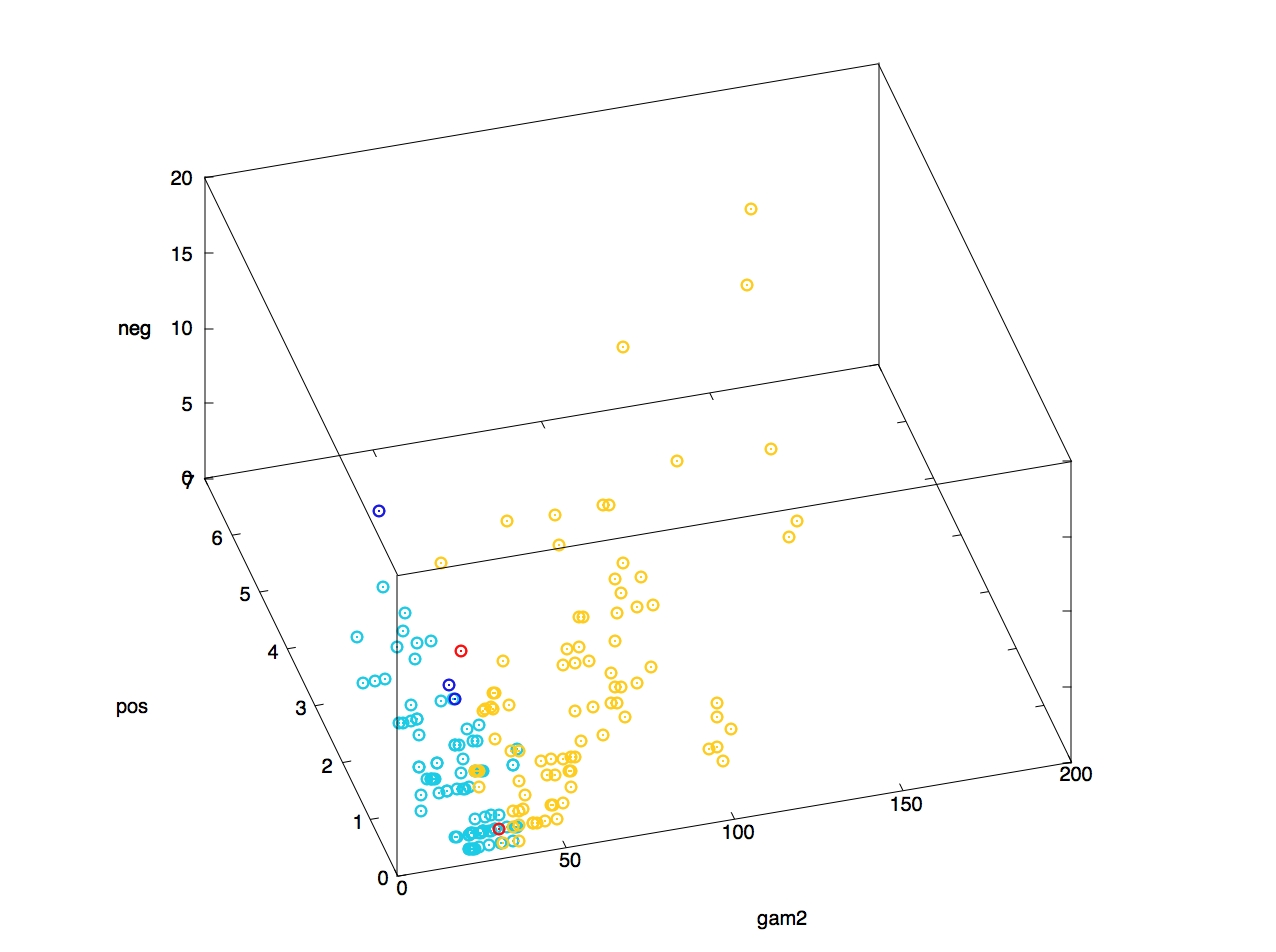
\includegraphics[width=1\textwidth]{naiverBayes}
\caption{Ergebnis der Pr\"ufung des naiven Bayes-Klassifikators}
\end{figure}

\begin{figure}[ht]
\centering
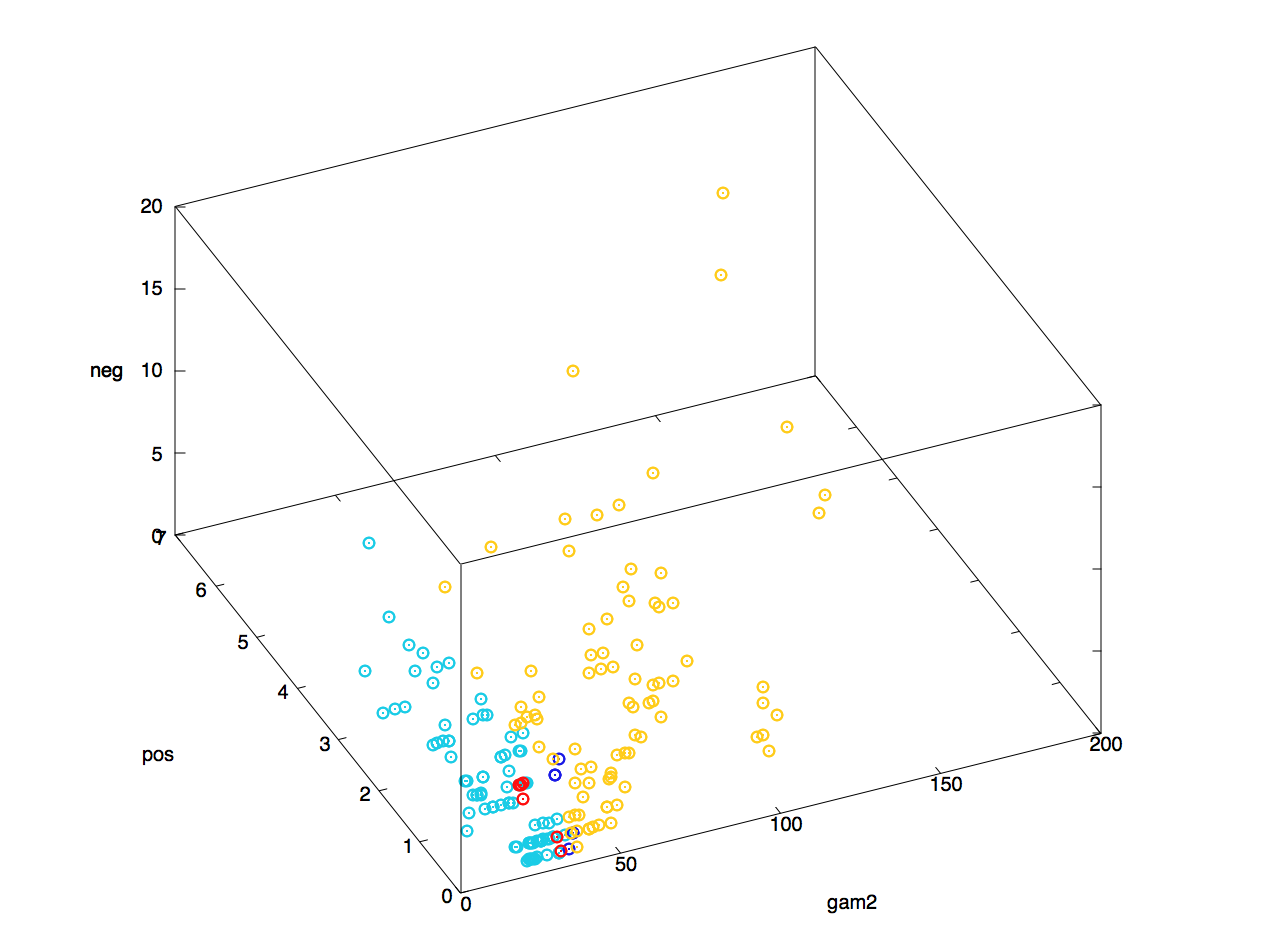
\includegraphics[width=1\textwidth]{neuronalesNetz}
\caption{Ergebnis der Pr\"ufung des neuronalen Netzes}
\end{figure}
\chapter{Mustererkennung}

\paragraph{}
Unter dem Begrif\mbox{}f Mustererkennung versteht man die auomatische
Verarbeitung und Auswertung von Mustern und deren Zuordnung zu vorbestimmten
Klassen. Die Muster erkennung setzt eine problemangepa\ss{}te Mess%
weterfassung voraus. Bild \ref{fig:mustererkennung} zeigt die Struktur eines
akustischen \cite{mekonnen92} Mustererkennungssytems.

\begin{figure}[ht]
\centering
\includegraphics[width=1\textwidth]{musterErkennung}
\caption{Struktur der Mustererkennung}
\label{fig:mustererkennung}
\end{figure}

\paragraph{}
Das \textbf{Messobjekt} ist der zu erkennende Gegenstand. In der 
Ger\"auschdiagnose werden Messbjekte nach einem bestimmten akustischen
Verhalten untersucht.

\paragraph{}
Der \textbf{Sensor} (Messwertaufnehmer) wandelt die vom Messobjekt
ausgestrahlten mechanischen oder akustischen Schwingungen (Messsignale) in
elektrische Signale um. Wegen ihrer Unempfindlichkeit gegen\"uber
Umgebungsger\"auschen werden bevorzugt K\"orperschallaufnehmer f\"ur die
Messwerterfassung eingesetzt.

\paragraph{}
Durch die \textbf{Vorverarbeitung} wird ein Signal in eine f\"ur die weitere
Verarbeitung geeignetere Form gebracht. Sie beinhaltet im wesentlichen die
AD-Wandlung des analogen elektrischen Signals und die Transformation in
geeignete Kennfunktionen. Dabei mu\ss{} eine optimale Aussteuerung des
AD-Wandlers gew\"ahrleistet sein. Dementsprechend m\"ussen Verst\"arkungs-
bzw. D\"ampfungsma\ss{}nahmen durchgef\"uhrt werden. Au\ss{}erdem sind die
Bedingungen des Abtasttheorems zu erf\"ullen, was gegebenenfalls den Einsatz
eines Antialiasing-Filters erfoldert.

\paragraph{}
Auf der Stufe der \textbf{Merkmalsextraktion} werden aus den Kennfunktionen
zun\"achst Kennwerte ermittelt, die Beitr\"age zur Klassentrennung liefern
k\"onnen. Um den Merkmalen Chancengleichheit bez\"uglich der Klassentrennung
einzur\"aumen, erfolgt h\"aufig eine Kennwertnormierung (z.B. in den Werte%
bereich [0..1]). Eine weitere Hauptaufgabe der Merkmalsextraktion ist die
Auswahl der signifikantesten Merkmale hinsichtlich ihrer Klassentrennungs%
f\"ahigkeit, die eine Merkmalsselektion bedeutet. Mit der Auswahl der Merkmale
ist eine Datenreduktion (Merkmalsreduktion) verbunden. Zus\"atzlich kann eine
Merkmalsreduktion liefert schlie\ss{}lich Merkmalsvektoren, die als Komponenten
die verschiedenen Merkmale bzw. deren Transformation enthalten.

\paragraph{}
Der Merkmalsvektor wird dem \textbf{Klassifikator} zur Verf\"ugung gestellt.
Dieser allein ist f\"ur eine Klassifikation nicht ausreichend. Ein Muster%
erkennungssystem kann eine Erkennungsaufgabe nur dann automatisch l\"osen,
wenn es bestimmte Informationen \"uber das zu erkennende Objekt und die zu
differenzierenden Klassen besitzt. Der Klassifikator ben\"otigt also f\"ur die
Zuordnung des Messobjektes zu einer Lernphase zu berechnen sind. Die Art der
klassenspezifischen Information h\"angt vom verwendeten Klassifikatortyp ab. Je
nach Art der Entscheidungsfunktion kann es sich dabei um eine Stichprobe
vorklassifizierter Muster oder um Klassenrepr\"asentanten (Parameter) handeln,
die aus der Lernstichprobe berechnet werden. Falls keine Klassifikation eines
Messobjektes mit bestimmter Wahrscheinlichkeit m\"oglich ist, kann eine
R\"uckweisung erfolgen.\\
Um ein Urteil \"uber die Lernstichprobe zu bilden und die Eignung eines
Klassifikators f\"ur diese zu testen, wird die Lernstichprobe klassifiziert.
Dir Klassifikation der Lernmuster selbst, also der Proze\ss{} der Re%
klassifikation, liefert eine scheinbare Fehlerrate. Im Idealfall sollte
diese 0\% betragen. Diese sogenannte Reklassifikationsfehlerrate wird als
Akzeptanzma\ss{} daf\"ur angesehen, ob eine Lernstichprobe f\"ur die
Klassifikation unabh\"angiger Objekte geeignet ist.\\
Die Reklassifikationsfehlerrate ist nicht allein ausreichend, um die Leistung
der Mustererkennung mit dem gew\"ahlten Klassifikator zu beurteilen. Praktisch
geht man so vor, eine unabh\"angige Teststichprobe mit bekannter Klassen%
zugeh\"origkeit der Objekte neu zu klassifizieren. Dieser Vorgang wird \textbf{%
Testklassifikation} genannt. Die Fehlerrate der Testklassifikation ist ein
reales Fehlerma\ss{} f\"ur den eingesetzten Klassifikator und liegt in der Regel
h\"oher als die scheinbare Fehlerrate bei Reklassifikation. Damit l\"a\ss{}t
sich die Wirksamkeit eines Erkennungssystem beurteilen.
\chapter{Merkmalsbeschreibung}

\paragraph{}
Das Zeitsignal ist aus dem Sensor noch nicht f\"ur die Klassifikation verwendbar. Es muss deshalb zun\"achst die Transformation in geeignete Kennfunktionen erfolgen. Die Aufgabe der Merkmalsbildung besteht dann in der Erstellung eines Merkmalsvektors aus dem Zeitbereich und den verschiedenen Kennfunktionen, was gleichbedeutend mit Transformation der Kennfunktionen in den Merkmalsvektor ist.\\
Bei der Kennwertberechnung kann man verschiedene Ans\"atze verfolgen. So existieren Standardkennwerte zur Auswertung der Signalverl\"aufe. In dieser Arbeit wurden die Verfahren f\"ur die Kennwertberechnung aus den mehreren Quellen genommen. Die Wahl dieser Kennwerte muss hinsichtlich der Beitr\"age f\"ur eine Klassentrennung sinnvoll sein.

\section{Kennwertberechnung aus dem Zeitbereich}

\paragraph{}
Die Berechnung von Kennwerten im Zeitbereich erfolgt mit direktem Bezug auf die Abtastwerte. Im Zeitverlauf eines Signals sind Unterschiede zwischen schadhaften und schadfreien Objekte zu verzeichnen. Bei der Implementierung von Kennwerten wurden \"Uberlegungen angestellt, diese Unterschiede zu erfassen.

\paragraph{Spannweite der Schwingung (XSPA)\\}
Eine hohe Spannweite (Schwingungsbreite) zwischen den positiven und negativen Extremwerten charakterisiert ein lautes Ger\"ausch. Die schadhaften Objekte weisen gr\"o\ss{}ere Spannweiten auf.

\begin{equation}
\mathit{XSPA}=\mathit{XMAX}-\mathit{XMIN}
\end{equation}

\paragraph{Gleichrichtwert (XGRW)\\}
Der Gleichrichtwert ist der betragsm\"a\ss{}ige Mittelwert (Erwartungswert der Betr\"age). In der Ger\"auschanalyse stellt dieser Kennwert einen Pegelwert dar.

\begin{equation}
\mathit{XGRW} = \frac{1}{m}\sum_{i=1}^{m}|x^{(i)}|
\end{equation}

\paragraph{Effektivwert (XEFF)\\}
Der Effektivwert liefert eine Aussage \"uber die Leistung des gesamten Signals.

\begin{equation}
\mathit{XEFF}=\sqrt{ \frac{1}{m}\sum_{i=1}^{m}(x^{(i)})^{2}}
\end{equation}

\paragraph{Formfaktor (FFAK)\\}
Der Formfaktor (shape factor) ist eine verst\"arkungsunabh\"angiger Kennwert zur Beschreibung der Signalform. F\"ur eine Normalverteilung liegt dieser Kennwert bei etwa 1.25.

\begin{equation}
\mathit{FFAK}=\frac{\mathit{XEFF}}{\mathit{XGRW}}
\end{equation}

\section{Kennwertberechnung aus der Amplitudenverteilungsdichte}

\paragraph{}
Aus der Amplitudenverteilungsdichte (AVD) lassen sich Kennwerte berechnen, mit denen es m\"oglich ist, Wahrscheinlichkeitsaussagen \"uber die Verteilung zu treffen. W\"ahrend die Kennwerte der schadfreien Objekte ann\"ahernd der Normalverteilung gehorchen, weisen die Kennwerte der schadhaften Objekte eindeutige Abweichungen von der Normalvertelung auf. Diese Abweichungen k\"onnen mittels statistischer Kennwerte ermittelt werden. Die Berechnung der Kennwerte aus der AVD erfolgt mit Hilfe der Wahrscheinlichkeitsdichte $p^{(i)}$.

\paragraph{Zentralmomente (MOM2, MOM3, MOM4), $\mu_{g}$\\}
Dabei wird mit $\mu_{1}$ das erste Moment (arithmetischer Mittelwert) bezeichnet. F\"ur mittelwertfreie stochastische Schwingungen ist $\mu_{1}$ gleich Null. Aus den Zentralmomenten $\mu_{2}$ bis $\mu_{4}$ lassen sich weitere Kennwerte definieren, die die Verteilung beschreiben.

\begin{equation}
\mu_{g}=\sum_{i=1}^{m}p^{(i)}(i-\mu_{1})^{g}
\end{equation}

\paragraph{Schiefe (GAM1), $\Gamma_{1}$\\}
Die Schiefe $\Gamma_{1}$ ist ein Ma\ss{} f\"ur die Symmetrie der Verteilung.

\begin{equation} \label{eq:gam1}
\Gamma_{1}=\frac{\mu_{3}}{(\sqrt{\mu_{2}})^{3}}
\end{equation}

\paragraph{Exzess (GAM2), $\Gamma_{2}$\\}
Der Exzess $\Gamma_{2}$ gibt die Abweichung der Verteilung von der Normalverteilung an. F\"ur die schadfreie Objekte, deren AVD normalverteilt ist, liegt der Exzess bei 3. Er wird benutzt, um die Abweichung der AVD von der Normalverteilung zu erfassen.

\begin{equation} \label{eq:gam2}
\Gamma_{2}=\frac{\mu_{4}}{(\mu_{2})^{2}}
\end{equation}

\section{Kennwertberechnung aus dem Fourier-Bereich}

\paragraph{}
Ausgangspunkt f\"ur die Fourier-Kennwerte sind der Betrag der Daten nach der Fourier-Analyse. Die Diskrete Fourier-Transformation wird f\"ur die Bestimmung der in einem abgetasteten Signal haupts\"achlich vorkommenden Frequenzen verwendet (Bild \ref{fig:signalFourier}). Die Berechnung der Kennwerte aus dem Fourier-Bereich ist gleich wie aus der AVD, erfolgt mit Hilfe der Wahrscheinlichkeitsdichte $p^{(i)}$. Daraus lassen sich zwei Kennwerte berechnen: \textbf{Schiefe} (Gleichung \ref{eq:gam1}) und \textbf{Exzess} (Gleichung \ref{eq:gam2}).

\begin{figure}[ht]
\centering
\includegraphics[width=\textwidth]{signalInFourier}
\caption{Umwandlung des Signals mit der DFT}
\label{fig:signalFourier}
\end{figure}

\section{Kennwertberechnung aus dem ``Hill Pattern''}

\paragraph{}
Hill Pattern wurde in \cite{hills} entwickelt und noch in \cite{saowaluck} benutzt. Die Idee besteht darin, um  das urspr\"ungliche Signal mit dem Mittelwert zu vergleichen und dann einen neuen Wert zu jedem Punkt zu zuweisen (Bild \ref{fig:signalHills}):

\begin{itemize}
\item +1, wenn der Wert des Signals gr\"o\ss{}er als Mittelwert + Schwellwert ist;
\item --1, wenn der Wert des Signals kleiner als Mittelwert -- Schwellwert ist;
\item 0, wenn der Wert des Signals in [Mittelwert -- Schwellwert; Mittelwert + Schwellwert] liegt.
\end{itemize}

\begin{figure}[ht]
\centering
\includegraphics[width=\textwidth]{signalInHills}
\caption{Umwandlung des Signals mit dem ``Hill Pattern''}
\label{fig:signalHills}
\end{figure}

Im Ergebnis krieg man ``Hill Pattern'' von ``Spitzen'' und ``T\"aler'' in der Unterschrift des Fahrzeuges. In dieser Arbeit werden diese Merkmale \textbf{positive Spitzen} und \textbf{negative Spitzen} genannt.

\section{Merkmalsnormierung}
\paragraph{}
Der Unterschied in den Wertebereichen der berechneten Kennwerte ist sehr gro\ss{}. Durch die Mischung der Kennwerte aus den verschiedenen Kennfunktionen haben die Komponenten des Merkmalsvektors unterschiedliche Dimensionen. Bei der Klassifikation kommt es darauf an, die Komponenten des Merkmalsvektors gleichberechtigt einzusetzen. Ziel von Normierungsma\ss{}nahmen ist es, den Wertebereich einiger Parameter auf einen vorgegebenen Wert oder Wertbereich zu bringen. Da\"ur gibt es zwei Techniken: Feature-Skalierung und Mittelwert-Normalisierung. Bei der Feature-Skalierung wird das Eingangsmerkmal durch den Bereich (d.h. Maximalwert minus Minimalwert) dividiert. Die Mittelwert-Normalisierung zieht Mittelwert des Eingangsmerkmal aus jedem Wert. Die beide Techniken k\"onnen als Gleichung \ref{eq:normierung} geschrieben werden:

\begin{equation} \label{eq:normierung}
x_i := \frac{x_i - \mu_i}{s_i},
\end{equation}
wobei $\mu_i$ der Durchschnitt von allen Werten ist, und $s_i$ Maximum minus Minimum oder Standardabweichung ist.

\paragraph{}
In dieser Arbeit und \cite{mekonnen92} wurden best\"atigt, dass eine Datennormierung zu verbesserten Klassifikationsergebnissen f\"uhrt. Bei der Normierung muss man darauf achten, dass die Teststichprobe mit der Lernstichprobe normiert wird, d.h. $\mu_i$ und $s_i$ in Gleichung \ref{eq:normierung} m\"ussen aus der Lernstichprobe bestimmt werden.
\chapter{Algorithmen Beschreibung}

\section{K-Means}

\paragraph{}
Der K-Means Algorithmus ist am beliebtesten und am h\"aufigste verwendeter Algorithmus f\"ur die automatische Gruppierung der Daten in die koh\"arenten Untermengen.

\begin{enumerate}
\item Initialisieren die Clusterzentren -- zuf\"allige $K$ Punkte aus der Stichprobe.
\item Clusterzuordnung: jedes Muster wird zum n\"achsten Cluster geordnet, basierend auf dem Abstand zwischen dem Muster und dem Mittelpunkt vom Cluster.
\item Bewegung des Mittelpunktes: die Mittelwerte f\"ur alle Punkte innerhalb jedes Clusters werden berechnet, dann werden die Clusterzentren auf diesen Durchschnitt verschoben.
\item Wiederholen Sie 2. und 3. Schritte, bis wir unsere Clusters gefunden haben werden (Bild \ref{fig:kmeans}).
\end{enumerate}

\begin{figure}[ht]
\centering
\includegraphics[width=1\textwidth]{KMeans}
\caption{Darstellung von K-Means auf den 1. und 6. Iterationen}
\label{fig:kmeans}
\end{figure}

K-Means kann im lokalen Optimum stecken. Um die Chance dieses Falls zu reduzieren, kann der Algorithmus auf der verschiedenen zuf\"alligen Initialisierungen ausgef\"uhrt werden.

\paragraph{Optimierungsziel\\}
Einf\"uhren wir die folgende Parameter:
\begin{itemize}
\item $c^{(i)}$ -- Index des Clusters (1, 2, \dots, $K$), zu dem der Muster $x^{(i)}$ aktuell zugeordnet wird
\item $\mu_{k}$ -- Clusterzentrum $k$ ($\mu_{k} \in \mathbb{R}^{n}$)
\item $\mu_{c^{(i)}}$  -- Clusterzentrum des Clusters, zu dem der Muster $x^{(i)}$ zugeordnet wird
\end{itemize}

Diese Variablen verwenden, k\"onnen wir unsere Kostenfunktion definieren:
\begin{equation}
J(c^{(i)},\dots,c^{(m)},\mu_1,\dots,\mu_K) = \frac{1}{m}\sum_{i=1}^m ||x^{(i)} - \mu_{c^{(i)}}||^2
\end{equation}
Unsere Optimierungsziel ist es, alle Parameter mit Hilfe der oben genannten Kostenfunktion zu minimieren: $min_{c,\mu}\ J(c,\mu)$. Bei dem 2. Schritt minimieren wir $J(\dots)$ mit $c^{(1)},\dots,c^{(m)}$ ($\mu_1,\dots,\mu_K$ sind fest). Bei dem 3. Schritt minimieren wir $J(\dots)$ mit $\mu_1,\dots,\mu_K$. Mit K-Means ist es nicht m\"oglich, dass die Kostenfunktion teilweise erh\"oht. Sie muss immer absteigen.


\section{Neuronales Netz}

\paragraph{}
Neuronale Netze sind begrenzte Imitationen, wie unsere eigenen Gehirne arbeiten. Sie hatten ein gro\ss{}es Wiederaufleben in j\"ungster Zeit wegen der Fortschritte in der Computer-Hardware.
Bei einer sehr einfachen Ebene sind Neuronen im Grunde die Recheneinheiten, die die Eing\"ange (Dendriten) als die elektrische Eingabe (so genannte ``Spikes'') verwenden, die zu den Ausg\"angen (Axone) geleitet werden.

\paragraph{Modelldarstellung\\}
Das Neuron l\"asst sich als ein Knoten (Bild \ref{fig:neuron}) darstellen. Es hat die Eingangsmerkmale $(x_1 \dots x_n)$ als Dendriten. Die Unit $x_0$ ist immer 1 gleich und wird ``Bias-Unit'' genannt. Der Einfluss der Eingabe auf das Neuron wird durch den Gewichtsvektor $\Theta$ gesteuert. Input einer Unit lassen sich als Formeln darstellen:
\begin{equation}
z=\sum^n_{i=1}\Theta_ix_i=\bar{\Theta}^T\bar{x}.
\end{equation}

\begin{figure}[ht]
\centering
\includegraphics[width=0.8\textwidth]{neuron}
\caption{Modell des Neurons}
\label{fig:neuron}
\end{figure}

Die Ausgabe ist eine Aktivit\"atsfunktion oder eine Hypothese $h_{\Theta}(x)$, die stellt den Zusammenhang zwischen dem Netzinput und dem Aktivit\"atslevel eines Neurons dar. In dieser Arbeit wird die Sigmoidfunktion als Aktivit\"ats\-funktion benutzt:
\begin{equation}
g(z)=\frac{1}{1 + e^{-z}}.
\end{equation}
Sie wird in einem 2-dimensionalen Diagramm (Bild \ref{fig:sigmoid}) visualisiert, wobei auf der x-Achse der Netzinput der Einheit und auf der y-Achse der entsprechende Aktivit\"atslevel abgetragen wird.

\begin{figure}[ht]
\centering
\includegraphics[width=0.9\textwidth]{sigmoid}
\caption{Sigmoidfunktion $g(z)$}
\label{fig:sigmoid}
\end{figure}

Neuronale Netze bestehen aus mehreren Neuronen. Diese Neuronen k\"onnen Informationen nicht nur aus der Umwelt, aber auch von anderen Neuronen aufnehmen, und an andere Units oder die Umwelt in modifizierter Form weiterleiten. Als Beispiel wird ein Netz betrachtet, das aus der Eingangs-, verdeckten und Ausgangsschicht besteht (Bild \ref{fig:neuNetz}). Neuronen der verdeckten Schichten und der Ausgangsschicht werden wie $a_i^{(j)}$ gekennzeichnet, wobei $i$ die Nummer des Neurons ist und $j$ die Nummer der Schicht ist. $\Theta^{(j)}$ ist eine Gewichtsmatrix f\"ur den \"Ubergang von der $j$ auf die $j+1$ Schicht.

\begin{figure}[ht]
\centering
\includegraphics[width=0.9\textwidth]{neuralNetwork}
\caption{Beispiel des Netzes}
\label{fig:neuNetz}
\end{figure}

Die Werte der Knoten werden wie folgt erhalten:
\begin{align*}
&a_1^{(2)} = g(\Theta_{10}^{(1)}x_0 + \Theta_{11}^{(1)}x_1 + \Theta_{12}^{(1)}x_2 + \Theta_{13}^{(1)}x_3) \\
&a_2^{(2)} = g(\Theta_{20}^{(1)}x_0 + \Theta_{21}^{(1)}x_1 + \Theta_{22}^{(1)}x_2 + \Theta_{23}^{(1)}x_3) \\
&a_3^{(2)} = g(\Theta_{30}^{(1)}x_0 + \Theta_{31}^{(1)}x_1 + \Theta_{32}^{(1)}x_2 + \Theta_{33}^{(1)}x_3) \\
&h_\Theta(x) = a_1^{(3)} = g(\Theta_{10}^{(2)}a_0^{(2)} + \Theta_{11}^{(2)}a_1^{(2)} + \Theta_{12}^{(2)}a_2^{(2)} + \Theta_{13}^{(2)}a_3^{(2)})
\end{align*}

Um Gewichtsmatrizen zu bestimmen, muss das Netz trainiert werden. In dieser Phase lernt das neuronale Netz anhand des vorgegebenen Lernmaterials. Dementsprechend werden in der Regel die Gewichte zwischen den einzelnen Neuronen modifiziert. In dieser Arbeit als Lernalregel wird Backpropagation verwendet.

\paragraph{Kostenfunktion\\}
Die Genauigkeit der Hypothesis kann durch die Kostenfunktion gemessen werden. F\"ur ihre Bestimmung werden die folgende Variablen eingef\"uhrt:
\begin{itemize}
\item $L$ -- Gesamtzahl der Schichten in dem Netzwerk
\item $s_l$ -- Anzahl von Units (ohne Bias-Unit) in der Schicht $l$
\item $K$ -- Anzahl von Output-Units/Klassen
\end{itemize}
Die Gleichung der Kostenfunktion hat die folgende Form:
\begin{align}
J(\Theta) = &- \frac{1}{m} \sum_{i=1}^m \sum_{k=1}^K \left[y^{(i)}_k \log ((h_\Theta (x^{(i)}))_k) + (1 - y^{(i)}_k)\log (1 - (h_\Theta(x^{(i)}))_k)\right] \nonumber \\
&+ \frac{\lambda}{2m}\sum_{l=1}^{L-1} \sum_{i=1}^{s_l} \sum_{j=1}^{s_{l+1}} ( \Theta_{j,i}^{(l)})^2
\end{align}

\paragraph{Backpropagation\\}
Bei Netzen mit Hidden-Units gibt es ein Problem, dass man keinen direkten Fehler f\"ur Neuronen der Hidden-Schicht bestimmen kann. Dieses Problem entsteht, weil man nur f\"ur die Output-Schicht, nicht aber f\"ur die Hidden-Schicht den gew\"unschten Output kennt und hieraus (zusammen mit dem tats\"achlichen Output) einen Fehlerterm ermitteln kann. Um dennoch eine Modifikation der Gewichte \"uber die entstehenden Fehlerterme vornehmen zu k\"onnen wird in der Trainingsphase jede Gewichtsver\"anderung in drei Schritte unterteilt:
\begin{enumerate}
\item Forward-Pass: Zun\"achst werden - wie in der Trainings- und der Testphase \"ublich - den Input-Neuronen Reize pr\"asentiert und sodann der Output des neuronalen Netzes berechnet.
\item Fehlerbestimmung: In einem zweiten Schritt erfolgt die Fehlerbestimmung f\"ur die Output-Units, indem die gew\"unschten Output-Werte mit den im forward-pass tats\"achlich ermittelten Werten verglichen werden. Wenn die Fehler eine vorgegebene G\"uteschwelle \"uberschreiten, folgt der dritte Schritt. Sind die Fehler klein genug und \"uberschreiten die G\"uteschwelle nicht, kann die Trainingsphase abgebrochen werden.
\item Backward-Pass: Der dritte Schritt ist der innovative Kern des Backpropagation Verfahrens. Die Fehlerterme breiten sich nun in entgegengesetzter Richtung bis zur Input-Schicht aus. Mit Hilfe dieser Fehlerterme werden nun nach und nach (d.h. zun\"achst zwischen Output und letzter Hidden-Schicht, dann zwischen letzter und vorletzter Hidden-Schicht usw.) die Gewichte des Netzes modifiziert so dass die Fehlerterme kleiner werden.
\end{enumerate}

\section{Dimensionsreduktion}

\paragraph{}
Es gibt zwei Gr\"unde, um Dimensionsreduktion zu verwenden:

\begin{enumerate}
\item Wir haben viele redundante Daten. Dimensionsreduktion wird die gesamte Daten, die im Rechnerspeicher speichern, reduzieren und den Lernalgorithmus beschleunigen.
\item Visualisierung der Daten, die mehr als drei Dimensionen ist. Wir k\"onnen die Dimensionen unserer Daten zu drei oder weniger reduzieren, um es zu zeichnen.
\end{enumerate}

Wir brauchen neue Merkmale zu finden ($z_{1}$, $z_{2}$ und $z_{3}$, z.B.), die alle anderen Merkmale effektiv zusammenfassen k\"onnen.\\
Der beliebtester Algorithmus der Dimensionsreduktion ist \textit{Principal Component Analysis (PCA)}.

\paragraph{Problembeschreibung\\}
Als Beispiel, es gibt zweidimensionaler Merkmalsraum, der aus $x_{1}$ und $x_{2}$ besteht. Man braucht eine Linie zu finden, die beide Merkmale gleichzeitig effektiv beschreibt. Daf\"ur muss man eine Richtung finden, darauf Daten zu projizieren, um den Projektions-Fehler zu minimieren.

\paragraph{}
PCA ist nicht lineare Regression (Bild \ref{fig:pcareg}). Bei der linearen Regression wird der quadrierte Fehler von jedem Punkt bis die Vorhersage Linie minimiert. Das ist der vertikale Abstand. Bei dem PCA Algorithmus der orthogonale Abstand wird minimiert. Wir nehmen die Merkmale und finden unter ihnen am n\"achsten gemeinsamen Datensatz. Wir versuchen, kein Ergebnis zu prognostizieren, und wir wenden keine Theta-Gewichte zu den Merkmalen.

\begin{figure}[ht]
\centering
\includegraphics[width=1\textwidth]{PCA}
\caption{Unterschied zwischen dem PCA und der linearen Regression}
\label{fig:pcareg}
\end{figure}

\paragraph{Algorithmus}

\begin{enumerate}

\item Berechnen ``Kovarianzmatrix''
\begin{equation}
\Sigma = \frac{1}{m}\sum^m_{i=1}(x^{(i)})(x^{(i)})^T
\end{equation}
$X$ ist eine $m \times n$ Matrix (die zeilenweise gespeicherte Muster), und das Produkt von denen wird eine $n \times n$ Matrix.

\item Berechnen ``Eigenvektoren'' von Kovarianzmatrix $\Sigma$\\
Dazu gibt es in Octave eine eingebaute Funktion, \textit{svd} oder `singular value decomposition' (Einzelwertzerlegung). Sie gibt drei Variable zur\"uck, aus der wir nur die erste, die Matrix U brauchen. 

\item Projizieren die Daten auf die $k$ Eigenvektoren\\
Aus der Matrix U werden die erste $k$ Spalten genommen, das wird $n \times k$ Matrix sein. Dann multiplizieren wir das mit der Merkmalsmatrix $X$. Als Ergebnis bekommen wir $n \times k$ Matrix $z$ -- die Projektion von $X$ auf den $k$-dimensionalen Raum.

\end{enumerate}

Zusammenfassend wird der gesamte Algorithmus in Listing \ref{lst:PCA} gr\"oblich beschrieben. Vor  der Anwendung des Algorithmus ist es wichtig, Merkmal Skalierung und mittlere Normalisierung zu machen (Gleichung \ref{eq:normierung}).

\begin{lstlisting}[caption={PCA Algorithmus},label={lst:PCA}]
Sigma = (1/m) * X' * X;  % Berechnung der Kovarianzmatrix
[U,S,V] = svd(Sigma);    % Berechnung der projizierten Richtungen
Ureduce = U(:,1:k);      % Nehmen die erste k Richtungen
z = Ureduce' * x;        % Berechnung der projizierten Datenpunkte
\end{lstlisting}
\bibliography{literatur}

\end{document}